\documentclass{standalone}

\usepackage{tikz}
\usepackage{tkz-euclide}
\usetikzlibrary{calc}
\usetikzlibrary{positioning}
\usetikzlibrary{arrows.meta}
\usetikzlibrary{shapes,snakes}

\usepackage{times}

\definecolor{myblue}{rgb}{0.0,0.5,0.8}

\begin{document}
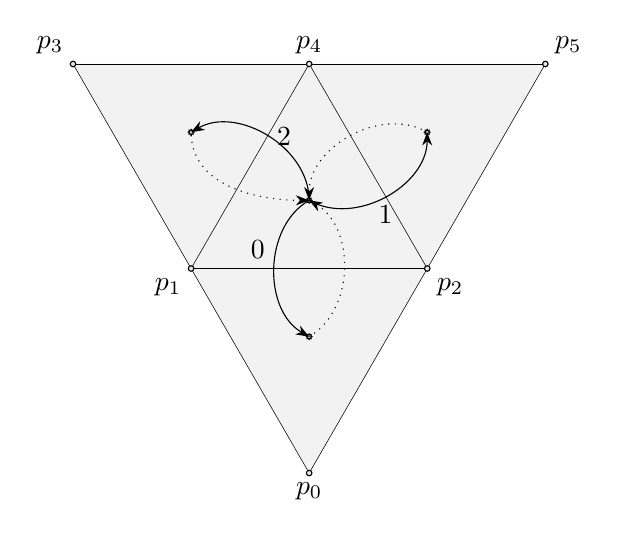
\begin{tikzpicture}[%
  >={Stealth[scale=1.0]},
  face/.style={star, star points = 8},
  scale=1.5,
]

  \tkzDefPoint(0.0, 0.0){v0}
  \tkzDefPoint(2.0, 0.0){v1}
  \tkzDefPoint(1.0, 1.7321){v2}
  \tkzDefPoint(1.0, -1.7321){v3}
  \tkzDefPoint(3.0, 1.7321){v4}
  \tkzDefPoint(-1.0, 1.7321){v5}

  \tkzFillPolygon[color=black!5](v0,v1,v2)
  \tkzFillPolygon[color=black!5](v0,v1,v3)
  \tkzFillPolygon[color=black!5](v1,v2,v4)
  \tkzFillPolygon[color=black!5](v2,v0,v5)

  \tkzDrawSegments(v0,v1 v1,v2 v2,v0 v0,v3 v3,v1 v1,v4 v4,v2 v2,v5 v5,v0)

  \tkzDrawPoints(v0,v1,v2,v3,v4,v5)

  \tkzDefTriangleCenter[in](v0,v1,v2)\tkzGetPoint{f0}
  \tkzDefTriangleCenter[in](v0,v1,v3)\tkzGetPoint{f1}
  \tkzDefTriangleCenter[in](v1,v2,v4)\tkzGetPoint{f2}
  \tkzDefTriangleCenter[in](v2,v0,v5)\tkzGetPoint{f3}
  \tkzDrawPoints[face](f0,f1,f2,f3)

  % \path[->,myblue,line width=0.8mm] (e0) edge[out=-90,in=90] node {} (te1);
  \path[->] (f0) edge[out=-150,in=150] node[above left] {$0$} (f1);
  \path[<-,dotted] (f0) edge[out=-30,in=30] node[below right] {} (f1);

  \path[->] (f0) edge[out=-30,in=-90] node[below] {$1$} (f2);
  \path[<-,dotted] (f0) edge[out=90,in=150] node[above right] {} (f2);

  \path[->] (f0) edge[out=90,in=30] node[right] {$2$} (f3);
  \path[<-,dotted] (f0) edge[out=180,in=-90] node[left] {} (f3);

  \tkzLabelPoint[below left](v0){$p_1$}
  \tkzLabelPoint[below right](v1){$p_2$}
  \tkzLabelPoint[above](v2){$p_4$}
  \tkzLabelPoint[below](v3){$p_0$}
  \tkzLabelPoint[above right](v4){$p_5$}
  \tkzLabelPoint[above left](v5){$p_3$}

\end{tikzpicture}
\end{document}
